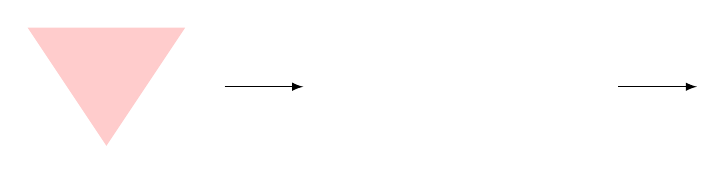
\begin{tikzpicture}
      \fill[opacity = 0.2, red] (2, 0) -- (1, 1.5) -- ( 3, 1.5) -- cycle; 
      \Vertex[x=0, y=0, size=0.25, fontscale=0.75, label=1]{v1}
      \Vertex[x=2, y=0, size=0.25, fontscale=0.75,label=2]{v2}
      \Vertex[x=1, y=1.5, size=0.25,fontscale=0.75, label=3]{v3}
      \Vertex[x=3, y=1.5, size=0.25,fontscale=0.75, label=4]{v4}
      \Edge(v1)(v2)
      \Edge(v1)(v3)
      \Edge(v2)(v3)
      \Edge(v2)(v4)
      \Edge(v3)(v4)

      \draw[-latex] ( 3.5, 0.75) -- (4.5, 0.75) ;

      \Vertex[x=5, y=0, size=0.25, fontscale=0.75, label=1]{v1}
      \Vertex[x=7, y=0, size=0.25, fontscale=0.75,label=2]{v2}
      \Vertex[x=6, y=1.5, size=0.25,fontscale=0.75, label=3]{v3}
      \Vertex[x=8, y=1.5, size=0.25,fontscale=0.75, label=4]{v4}
      \Edge(v1)(v2)
      \Edge(v1)(v3)
      \Edge(v2)(v3)
      \Edge(v2)(v4)

      \draw[-latex] ( 8.5, 0.75) -- (9.5, 0.75) ;

      \Vertex[x=10, y=0, size=0.25, fontscale=0.75, label=1]{v1}
      \Vertex[x=12, y=0, size=0.25, fontscale=0.75,label=2]{v2}
      \Vertex[x=11, y=1.5, size=0.25,fontscale=0.75, label=3]{v3}
      \Edge(v1)(v2)
      \Edge(v1)(v3)
      \Edge(v2)(v3)

\end{tikzpicture}